\section{Modelagem de Aplicações Paralelas} \label{sec:modelagem}

A programação paralela possibilita utilizar ao máximo os recursos de \textit{hardware}. Com isso, muitos problemas antes impossíveis de serem solucionados podem ser executados sem muito esforço. A demanda de desempenho necessária para a realização de uma tarefa está relacionada com a quantidade de dados ou variáveis envolvidas durante o processamento e quais as operações pelas quais estes terão de passar até o resultado. Quanto mais eficiente for a implementação de um algoritmo, menor a demanda por desempenho.

Segundo Foster~\cite{foster1995designing}, a modelagem de um problema de forma paralela passa por quatro fases: o particionamento, a comunicação, o agrupamento e o escalonamento.

\begin{description}
\item[1) Particionamento] - Primeiramente, os dados são divididos de maneira que cada tarefa possa ser executada independentemente das demais. Com isso obtém-se a menor granularidade possível para cada tarefa.

\item[2) Comunicação] - Em um segundo momento, devido ao fato de os dados normalmente estarem inter-relacionados, é necessário que haja a troca de informações entre os processos. Nessa fase é definida a forma de comunicação paralela adotada, caso seja utilizado uma arquitetura multiprocessada.

\item[3) Agrupamento] - Em seguida, em uma terceira fase, as operações ou dados são agrupados a fim de realizar um melhor uso dos processadores. O objetivo dessa fase é aumentar a granularidade das operações realizadas por um único processador. Assim, operações que envolvam um conjunto de dados vizinho são executadas em um mesmo processador, diminuindo a interdependência entre os dados.

\item[4) Escalonamento] - Por fim, na quarta etapa, ocorre o mapeamento, que é a fase que define como serão distribuídas as tarefas entre os processadores. Essa distribuição busca casar a granularidade das tarefas com a capacidade de processamento dos processadores e a dependência entre os processos que se encontram em processadores distintos.

\end{description}

A Figura~\ref{fig:modelagemFoster} ilustra cada uma das etapas descritas anteriormente. Inicialmente um conjunto de dados é particionado. Posteriormente são destacadas as interações entre dois pontos vizinhos de granularidade fina. Após o agrupamento entre alguns pontos é feito um mapeamento, que distribui as tarefas entre 5 processadores ($P1,...,P5$).


\begin{figure}[!htbp]
	\centerline{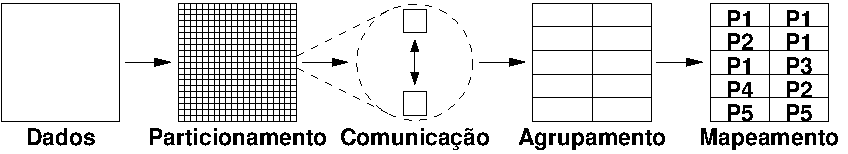
\includegraphics[scale=1.0]{modelagemFoster}}
	\caption{Principais etapas na paralelização de um algoritmo.}
	\label{fig:modelagemFoster}
\end{figure}

Mais conceitos de projeto e desenvolvimento de programas paralelos podem ser estudados no material base do minicurso Projetando e Construindo Programas Paralelos, apresentando na ERAD/RS 2019\footnote{https://www.setrem.com.br/erad2019/data/pdf/minicursos/mc02.pdf}.